

\documentclass[11pt,dvipdfmx]{beamer}

%%% 使用するテーマ(現在Copenhagenを指定しています。適当に変えてみよう。)%%%
%
\usetheme{Antibes}  
%\usetheme{Default}       % シンプルで機能的なテーマ #何も指定しない場合は自動的にこれ
%\usetheme{Bergen}        % フレームを縦方向に分割
%\usetheme{Boadilla}      % より多くの情報を収容可
%\usetheme{Madrid}        % Boadillaをよりカラフルにしたもの
%\usetheme{Pittsburgh}    % シンプルで機能的、見出しは右寄せ
%\usetheme{Rochester}     % 横方向のヘッダパネルが特徴     % 上部にナビゲーションバーを持つ、明瞭度の高いテーマ
%\usetheme{JuanLesPins}   % Antibesと類似のテーマ
%\usetheme{Montpellier}   % シンプルで色調のおとなしいもの
%\usetheme{Berkeley}      % 横方向のヘッダパネルを持つ機能的なテーマ
%\usetheme{PaloAlto}      % Berkeleyと類似のテーマ
%\usetheme{Goettingen}    % サイドバーは右側で、ヘッダパネルなし
%\usetheme{Marburg}       % Goettingenの色調を強くしたもの
%\usetheme{Hannover}      % サイドバーは左側で見出しは右寄せ
%\usetheme{Berlin}        % 縦方向のナビゲーションバーを上部に持つ強い色調のテーマ
%\usetheme{Ilmenau}       % Berlinと類似のテーマ
%\usetheme{Dresden}       % Ilmenauと類似のテーマ
%\usetheme{Darmstadt}     % 横方向のナビゲーションバーを上部に持つ
%\usetheme{Frankfurt}     % Darmstadtと類似、しかしサブセクション情報は含まない
%\usetheme{Singapore}     % ソフトな色調を持ったテーマ
%\usetheme{Szeged}        % Singaporeと類似、しかし境界線は明確
%\usetheme{Copenhagen}    % セクション/サブセクションテーブルを上部に配置
%\usetheme{Luebeck}       % Copenhagenから丸みを取ったもの
%\usetheme{Malmoe}        % Copenhagenをより質素にしたもの
\usetheme{Warsaw}        % Copenhagenと類似のテーマ

%%% 数式のフォント(TeXっぽいフォントになる)%%%
%
\usefonttheme{professionalfonts}


%%% 隠蔽されている要素の透明度の設定 %%%
%
%\setbeamercovered{transparent=10}

%%% その他のクラス・パッケージの導入 %%%

\usepackage{graphicx}  % includegraphicsコマンドなどで図を表示するためのクラス
\usepackage{amsmath}   % プロ仕様の数学用のフォントI(AMSはアメリカ数学会)
\usepackage{amssymb}   % プロ仕様の数学用のフォントII(AMSはアメリカ数学会)
\usepackage{bm}        % 太字を表現するのに便利なクラス
\usepackage[absolute,overlay]{textpos}


\usepackage[all]{xy}
\usepackage{amsthm,amsmath,amssymb,comment}
\usepackage{float}
\usepackage{graphicx}
\usepackage{color}

%% ゴシック体にする
%\renewcommand{\kanjifamilydefault}{gt}

% フォントはお好みで
%\usepackage{txfonts}
%\mathversion{bold}                             %%% 数式を太字にする
\renewcommand{\familydefault}{\sfdefault}
\renewcommand{\kanjifamilydefault}{\gtdefault} %%% 日本語フォントを太字にする
%\setbeamerfont{title}{size=\large,series=\bfseries}
%\setbeamerfont{frametitle}{size=\large,series=\bfseries}
%\setbeamertemplate{frametitle}[default][center]
%\usefonttheme{professionalfonts} 
%
\newtheorem{proposition}{命題}
\newtheorem{assumption}{仮定}
\newtheorem{cor}{系}
\newtheorem{remark}{Remark}
\newtheorem{exercise}{Exercise}

\newtheorem{thm}{Theorem}[section] 
\newtheorem{theo}[thm]{Theorem}
\newtheorem{corr}[thm]{Corollary}
\newtheorem{prop}[thm]{Proposition}
\newtheorem{conj}[thm]{Conjecture}
\newtheorem*{mainthm}{Theorem}
\newtheorem{deflem}[thm]{Definition-Lemma}
\newtheorem{lem}[thm]{Lemma}
\theoremstyle{definition} 
\newtheorem{defn}[thm]{Definition}
\newtheorem{propdefn}[thm]{Proposition-Definition} 
\newtheorem{lemdefn}[thm]{Lemma-Definition} 
\newtheorem{thmdefn}[thm]{Theorem-Definition} 
\newtheorem{eg}[thm]{Example} 
\newtheorem{ex}[thm]{Example} 
\theoremstyle{remark}
\newtheorem{rem}[thm]{Remark}
\newtheorem{obs}[thm]{Observation}
\newtheorem{ques}[thm]{Question}
%\newtheorem{problem}[thm]{Problem}
\newtheorem{setup}[thm]{Set up}
\newtheorem{notation}[thm]{Notation}
\newtheorem{cl}{Claim}
\newtheorem{claim}{Claim}
\newtheorem{step}{Step}
\newtheorem*{clproof}{Proof of Claim}
\newtheorem{cln}[thm]{Claim}
\newtheorem*{ack}{Acknowledgements} 



%% 自分で定義したマクロ
\newcommand{\Sym}{{\rm Sym}}

\newcommand{\Sigmat}{\mbox{\boldmath\ensuremath{\Sigma}}}
\newcommand{\evec}{\mbox{\boldmath\ensuremath{e}}}
\newcommand{\ovec}{\mbox{\boldmath\ensuremath{0}}}
\newcommand{\xvec}{\mbox{\boldmath\ensuremath{x}}}
\newcommand{\e}{{\rm e}}
\newcommand{\dr}{{\rm d}}
\newcommand{\E}{{\mathbb E}}
\newcommand{\p}{{\mathbb P}}
\newcommand{\V}{{\mathbb V}}
\newcommand{\R}{\mathbb{R}}
\newcommand{\Z}{\mathbb{Z}}
\newcommand{\Q}{\mathbb{Q}} 
\newcommand{\N}{\mathbb{N}}
\newcommand{\C}{\mathbb{C}} 
\newcommand{\mP}{\mathbb{P}}
\newcommand{\mO}{\mathcal{O}}
\newcommand{\Sin}{\text{Sin}^{-1}} 
\newcommand{\Cos}{\text{Cos}^{-1}} 
\newcommand{\Tan}{\text{Tan}^{-1}} 
\newcommand{\invsin}{\text{Sin}^{-1}} 
\newcommand{\invcos}{\text{Cos}^{-1}} 
\newcommand{\invtan}{\text{Tan}^{-1}} 
\newcommand{\Area}{\text{Area}}
\newcommand{\vol}{\text{Vol}}


%%%%%%%%%%%%%%%%%%%%%%%%%%%%%%%%%%%%%%%%%%%%%%%%%%%%%%%%%%%%%%%%%%%%%%%%
%%%%%%%%%%%%%%%%%%%%%%%%%%%%%%%%%%%%%%%%%%%%%%%%%%%%%%%%%%%%%%%%%%%%%%%%

%% タイトルページの情報登録 %%
%% プレゼンテーションの表題の登録 
%% []で囲んだものは表題の略称, {}で囲んだ方が正式な表題
%% \title[タイトルの略称]{タイトル}


% 影もグラデーションも使わない block に
\setbeamertemplate{blocks}[default]
\setbeamercolor{block title}{fg=white,bg=blue!70!black}
\setbeamercolor{block body}{bg=blue!7} % 薄色の単色
% (影を使っているなら)↓も併用
% \setbeamertemplate{blocks}[rounded][shadow=false]


\begin{document}



\begin{frame}
\frametitle{タイル1. }
図1のようなチェス盤は, 図2のような2×1のタイルで埋め尽くすことができないことを示せ.

ただし2×1のタイルは重なり合ってはいけないしはみ出てはいけない.
\begin{figure}[htbp]
\begin{center}
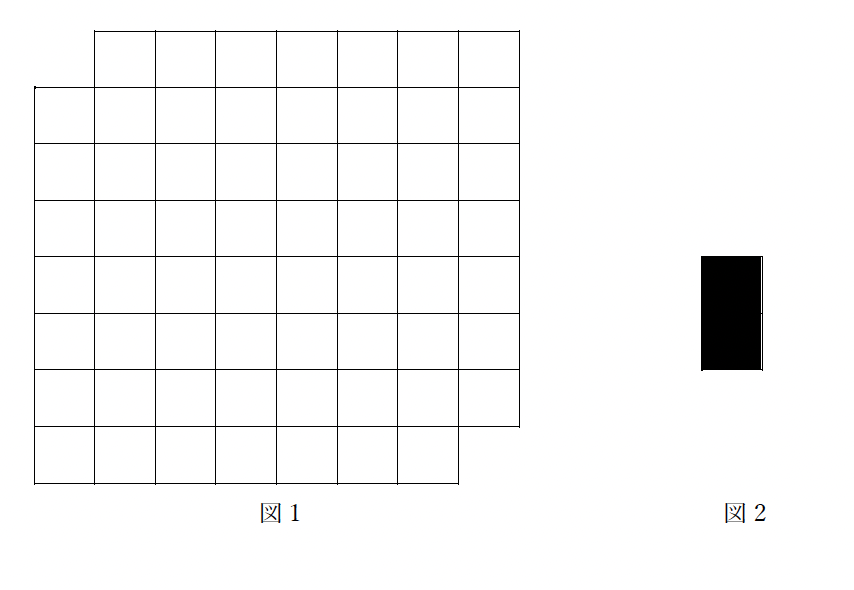
\includegraphics[width=80mm]{tile1.png}
\end{center}
\end{figure}
\end{frame}



\begin{frame}
\frametitle{タイル2. }
図1のような8×8のタイルの上に, 1×1タイルを好きなところにおく. 
このとき1×1タイルをどこにおいても, 図2のようなのタイルで埋め尽くすことができることを示せ.

ただし図2のようなタイルは重なり合ってはいけないしはみ出てはいけない.
\begin{figure}[htbp]
\begin{center}
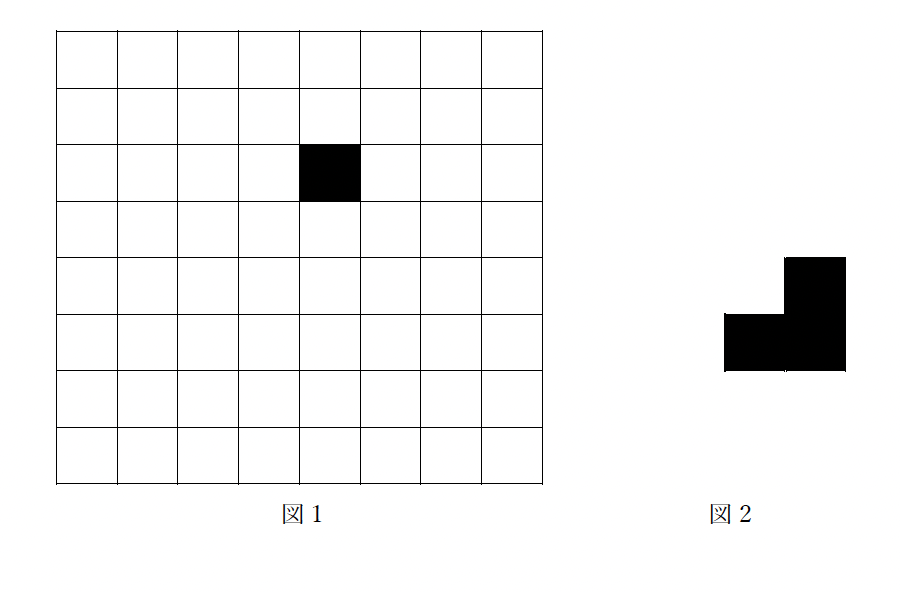
\includegraphics[width=80mm]{tile2.png}
\end{center}
\end{figure}
\end{frame}


\begin{frame}
\frametitle{タイル3. }
大きなタイルをたくさんの(有限個の)小さな長方形に分割した. 
その際全ての小さな長方形の縦の長さもしくは横の長さのどちらか(あるいは両方ともが)整数であった.

\vspace{5pt}
このとき, 大きな長方形の縦の長さもしくは横の長さのどちらか(あるいは両方とも)整数であることを示せ.
\begin{figure}[htbp]
\begin{center}
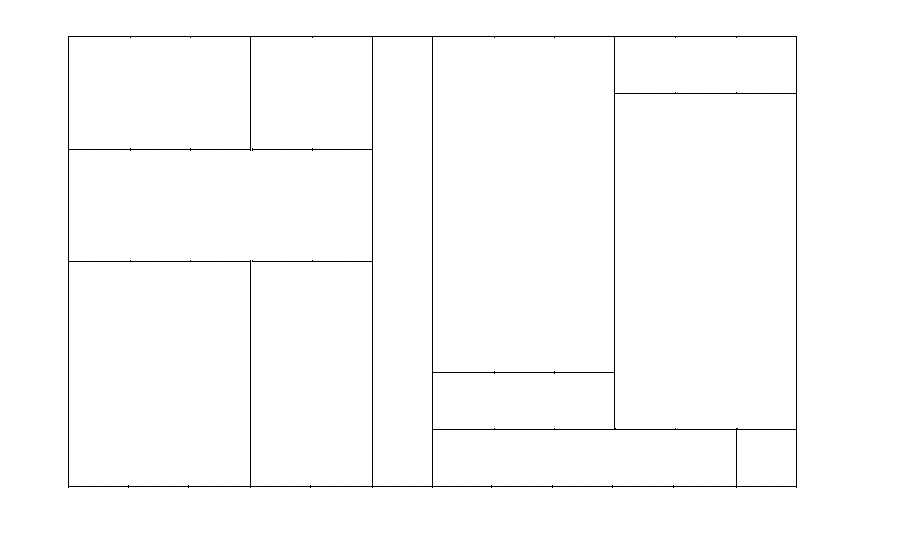
\includegraphics[width=70mm]{tile3.png}
\end{center}
\end{figure}
\end{frame}


\begin{frame}
\frametitle{Kontsevichのパズル}
図1のように, 左下の1枚だけを黒タイルとし, その他のタイルは白で, それらの白タイルが上方向と右方向に無限に並んでいるものを考える.
次の操作を何回やっても, 図2の赤色の部分に黒のタイルがあることを示せ. 

\vspace{5pt}
[操作] 図1のように上も右も白であるような黒のタイルを選び, それを白タイルに変えて, その上も右も黒のタイルに変える.

\begin{figure}[htbp]
\begin{center}
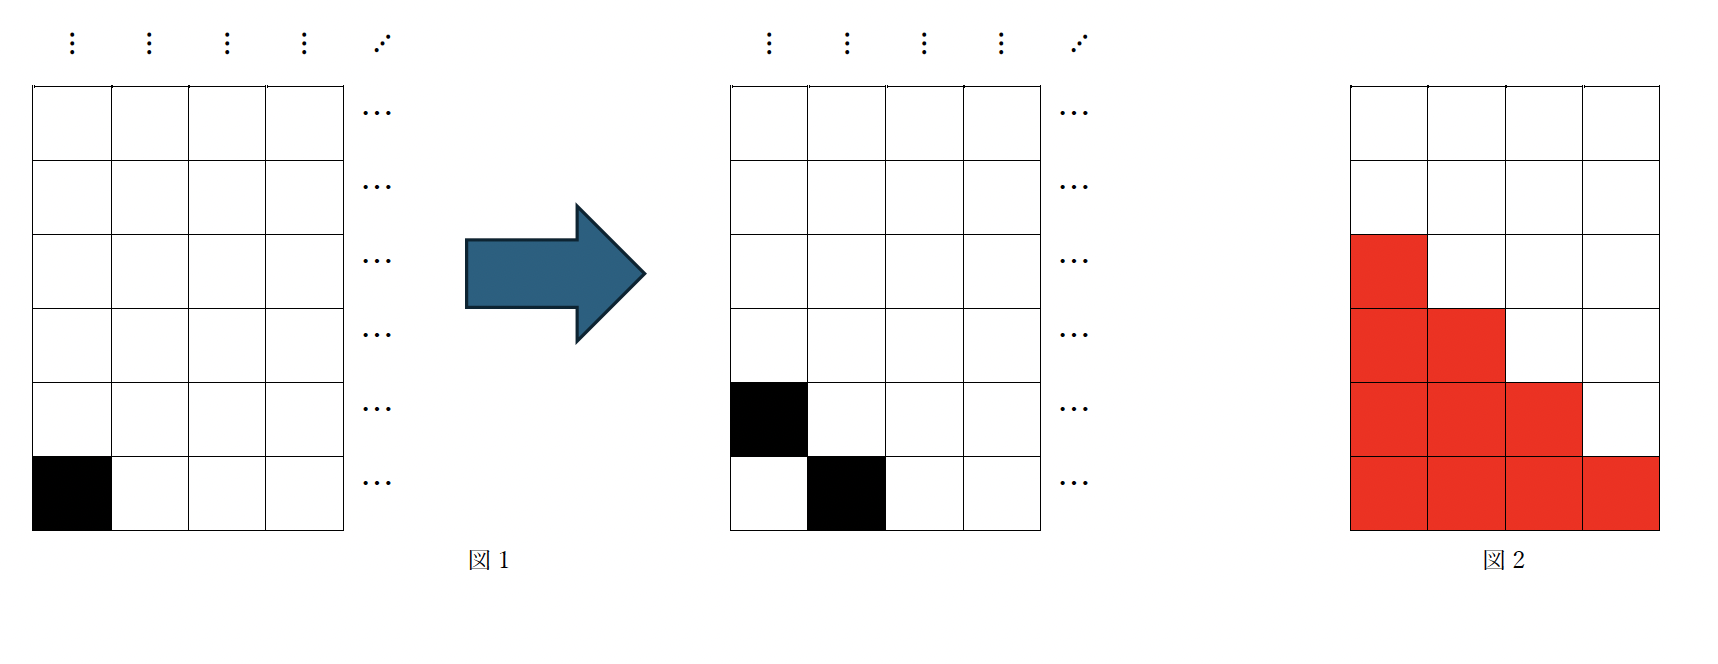
\includegraphics[width=100mm]{kont.png}
\end{center}
\end{figure}
\end{frame}





\begin{frame}
\frametitle{ドブル}
7色(赤, 橙, 黄, 緑, 青, 藍, 紫) のペンと7枚のカードある. 次のルールを考える.
\begin{enumerate}
    \setlength{\parskip}{0cm} 
  \setlength{\itemsep}{0cm} 
\item どのカードにも相異なる3 色の$\bullet$印がある.
\item どの2 枚のカードを取っても, 1 つだけ共通する色の$\bullet$印がある.
\end{enumerate}
上のルール2 つを満たすように色ペンを使ってカードに$\bullet$印を書くことはできるだろうか?

\vspace{20pt}
{\footnotesize
[補足] これをゲームにしたのがドブルである. ドブルで使うカードには, どんな2枚のカードを取っても共通する絵柄が必ず一つのみある. 
}

\end{frame}

\begin{frame}
\frametitle{$11111\cdots $}
$p$を2や5でない素数とする. 
$11111\cdots 111$という1が何個か並んだ形の$p$の倍数が存在することを示せ.

\vspace{20pt}
例えば...
\begin{itemize}
  \item $p=3$の場合は111は3の倍数.
  \item $p=7$の場合は111111は7の倍数.
  \item $p=11$の場合は11は11の倍数.
  \end{itemize}
\end{frame}


\begin{frame}
\frametitle{2010年大阪大学理系第3問}
$l,m,n$を3以上の整数とする. 等式
$$
\left( \frac{n}{m} - \frac{n}{2} + 1 \right)l = 2
$$
を満たす$l,m,n$の組を全て求めよ. 

\vspace{20pt}
{\footnotesize
[補足] 実はこの方程式は隣の部屋の展示物と大きな関連がある. 
}
\end{frame}

\begin{frame}
\frametitle{確率直感テスト}

皆さんの確率の直感がどれくらい当たっているかぜひ試してみてください. 

\begin{figure}[htbp]
\begin{center}

\includegraphics[width=70mm]{prob.png}
\end{center}
\end{figure}
\end{frame}


%2025/10/31追加
\begin{frame}
\frametitle{コイン 1}
テーブル上に10個の硬貨が一列に並んでいる. 
その硬貨の額は1円か5円か10円である. 

あなたと私の二人で次のルールの下, 以下のゲームを行う.

 \begin{block}{ルール}
\begin{itemize}
\item 列のうち左端か右端の硬貨を取る. その後次の人に手番をわたす.
\item テーブル上の硬貨がなくなった時, とった硬貨の総額が多い方が勝ち. 同じであれば引き分け. 
\end{itemize}
   \end{block}

ゲームに"負けたくない"あなたなら先手・後手どちらを選べば良いだろうか?
またその際どのような戦略を取れば良いだろうか?

\begin{figure}[htbp]
\begin{center}
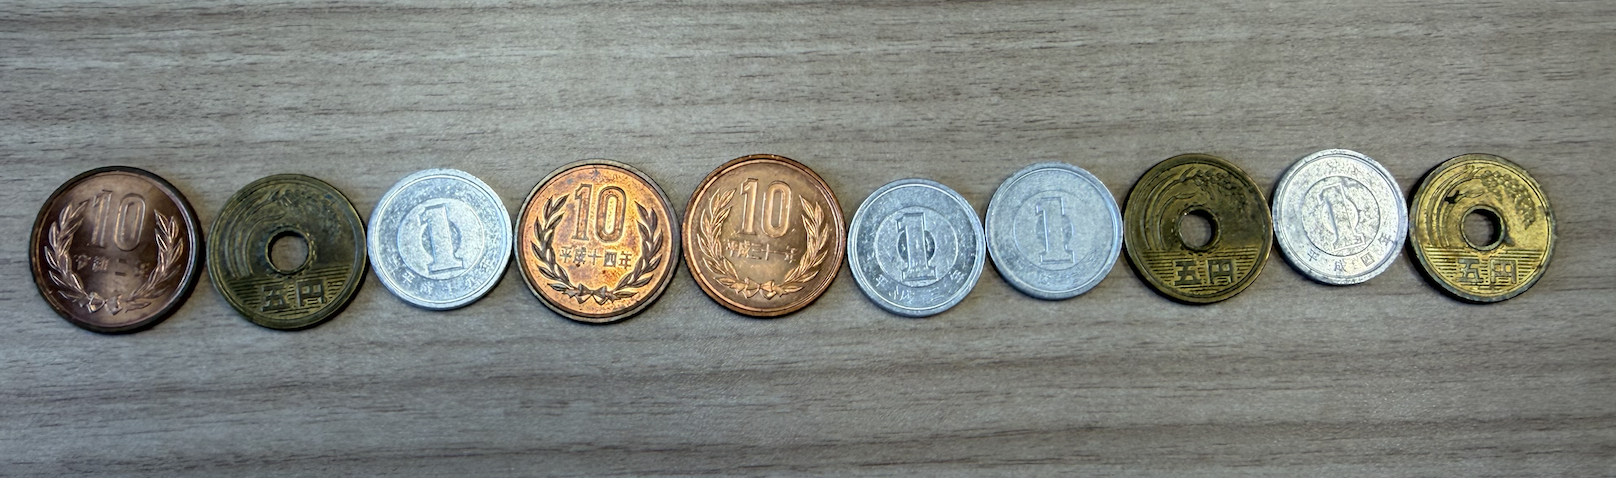
\includegraphics[width=80mm]{coin1.png}
\end{center}
\end{figure}

\end{frame}


\begin{frame}
\frametitle{コイン 2}
テーブル上に25個の1円玉がある.
あなたと私の二人で次のルールの下, 以下のゲームを行う.

 \begin{block}{ルール}
\begin{itemize}
\item テーブルの上の1円玉から, 1枚か2枚か3枚のコインを取る. その後次の人に手番をわたす. 
\item 最後の1円玉を取った人が負け.
\end{itemize}
   \end{block}

ゲームに"負けたくない"あなたなら先手・後手どちらを選べば良いだろうか?
またその際どのような戦略を取れば良いだろうか?

\begin{figure}[htbp]
\begin{center}
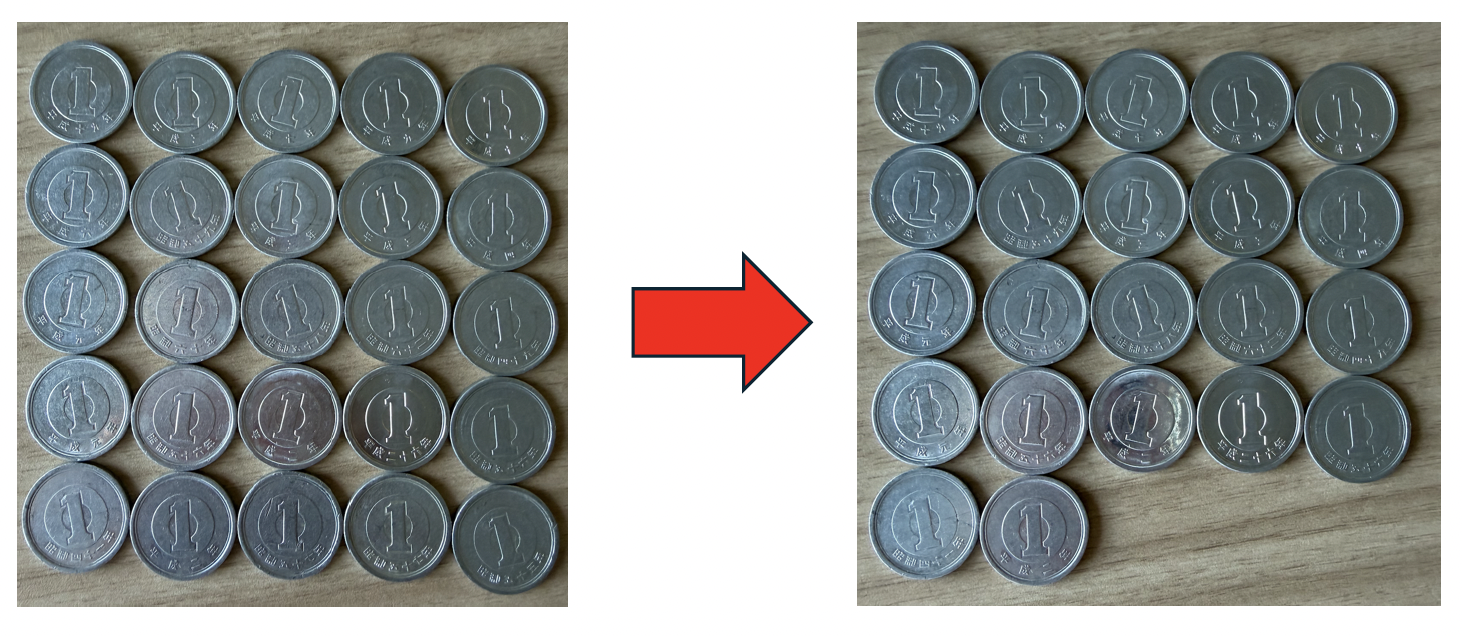
\includegraphics[width=80mm]{coin2.png}
\end{center}
\end{figure}

\end{frame}

\begin{frame}
\frametitle{コイン 2'}
テーブル上に25個の1円玉がある.
あなたと私の二人で次のルールの下, 以下のゲームを行う.

 \begin{block}{ルール}
\begin{itemize}
\item テーブルの上の1円玉から, \underline{1枚か3枚か4枚}のコインを取る. その後次の人に手番をわたす.
\item 最後の1円玉を取った人が負け.
\end{itemize}
   \end{block}

ゲームに"負けたくない"あなたなら先手・後手どちらを選べば良いだろうか?
またその際どのような戦略を取れば良いだろうか?


\end{frame}


\begin{frame}
\frametitle{コイン 3}
1円玉が裏向きに$5 \times 5$の正方形に並んでいる. 次の操作を考える. 
 \begin{block}{操作}
\begin{itemize}
\item 縦か横に連続する3枚の1円玉を同時にひっくり返す.
\end{itemize}
   \end{block}
 この操作を何回かして全ての1円玉を表向きにできるか?
 
 \begin{figure}[htbp]
\begin{center}
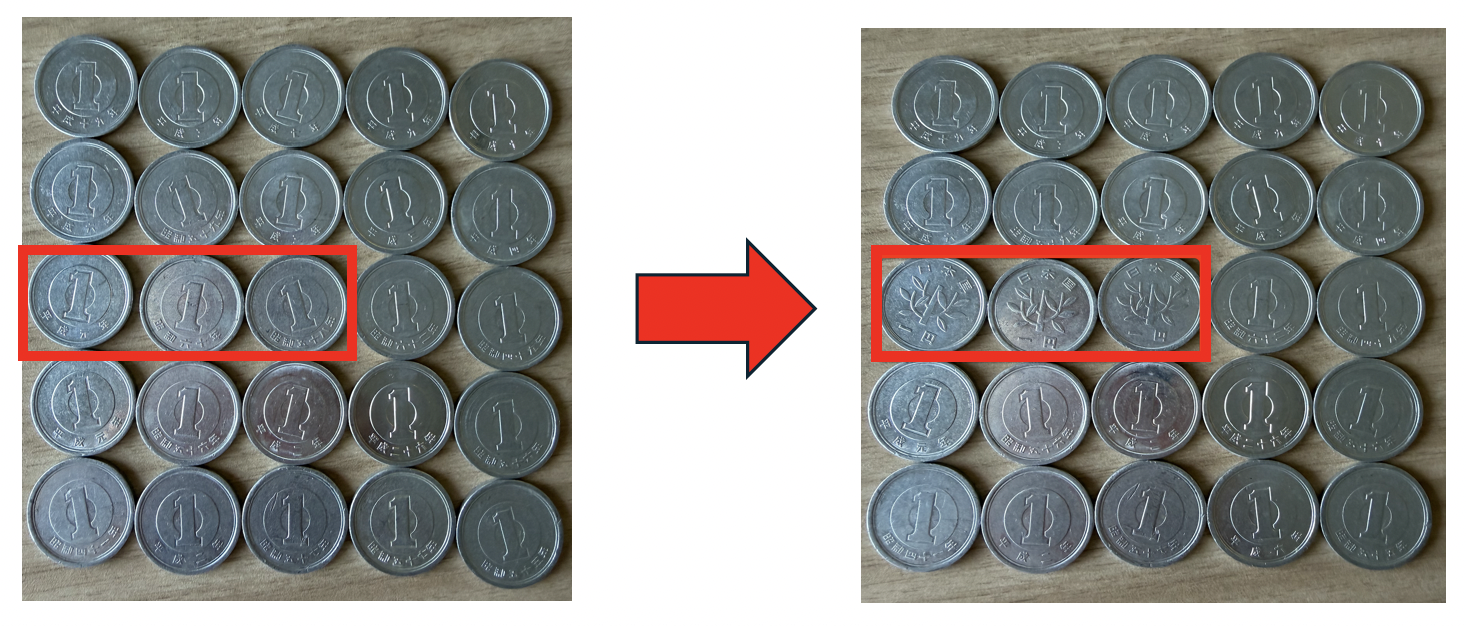
\includegraphics[width=80mm]{coin3.png}
\end{center}
\end{figure}

\end{frame}

\begin{frame}
\frametitle{$1 + \sqrt{2}$}
$(1 + \sqrt{2})^{2025}$の小数第100位を求めよ.
\end{frame}



\end{document}